\section{Methodology}\label{sec:Methodology}

\subsection{Motivation}\label{sec:Methodology:Motivation}
The existence of pseudo-change implies that reliable change detection requires both inter-temporal difference sensitivity and annotation-semantic consistency. In practical remote sensing datasets, visually changed regions may still be labeled as unchanged. Therefore, directly amplifying appearance discrepancy can lead to false positives and unstable generalization.

To address this issue, we design an annotation-consistency-oriented training strategy with two coupled components: (1) pseudo-change suppression in feature space via label-guided contrastive supervision, and (2) bounded multi-task joint optimization for segmentation, edge, and contrastive branches. This design shifts the objective from pure visual difference response to benchmark-consistent change prediction.

\subsection{Overview}\label{sec:Methodology:Overview}
Fig.~\ref{fig:method_overview} illustrates the full training pipeline. Two temporal images are first encoded by a shared backbone, then fused by pyramid-level temporal interaction to produce change and edge prediction branches. In parallel, deep temporal features are extracted for the \textsc{MarginalDistance} process to form a label-guided contrastive supervision signal.

\begin{figure*}[t]
    \centering
    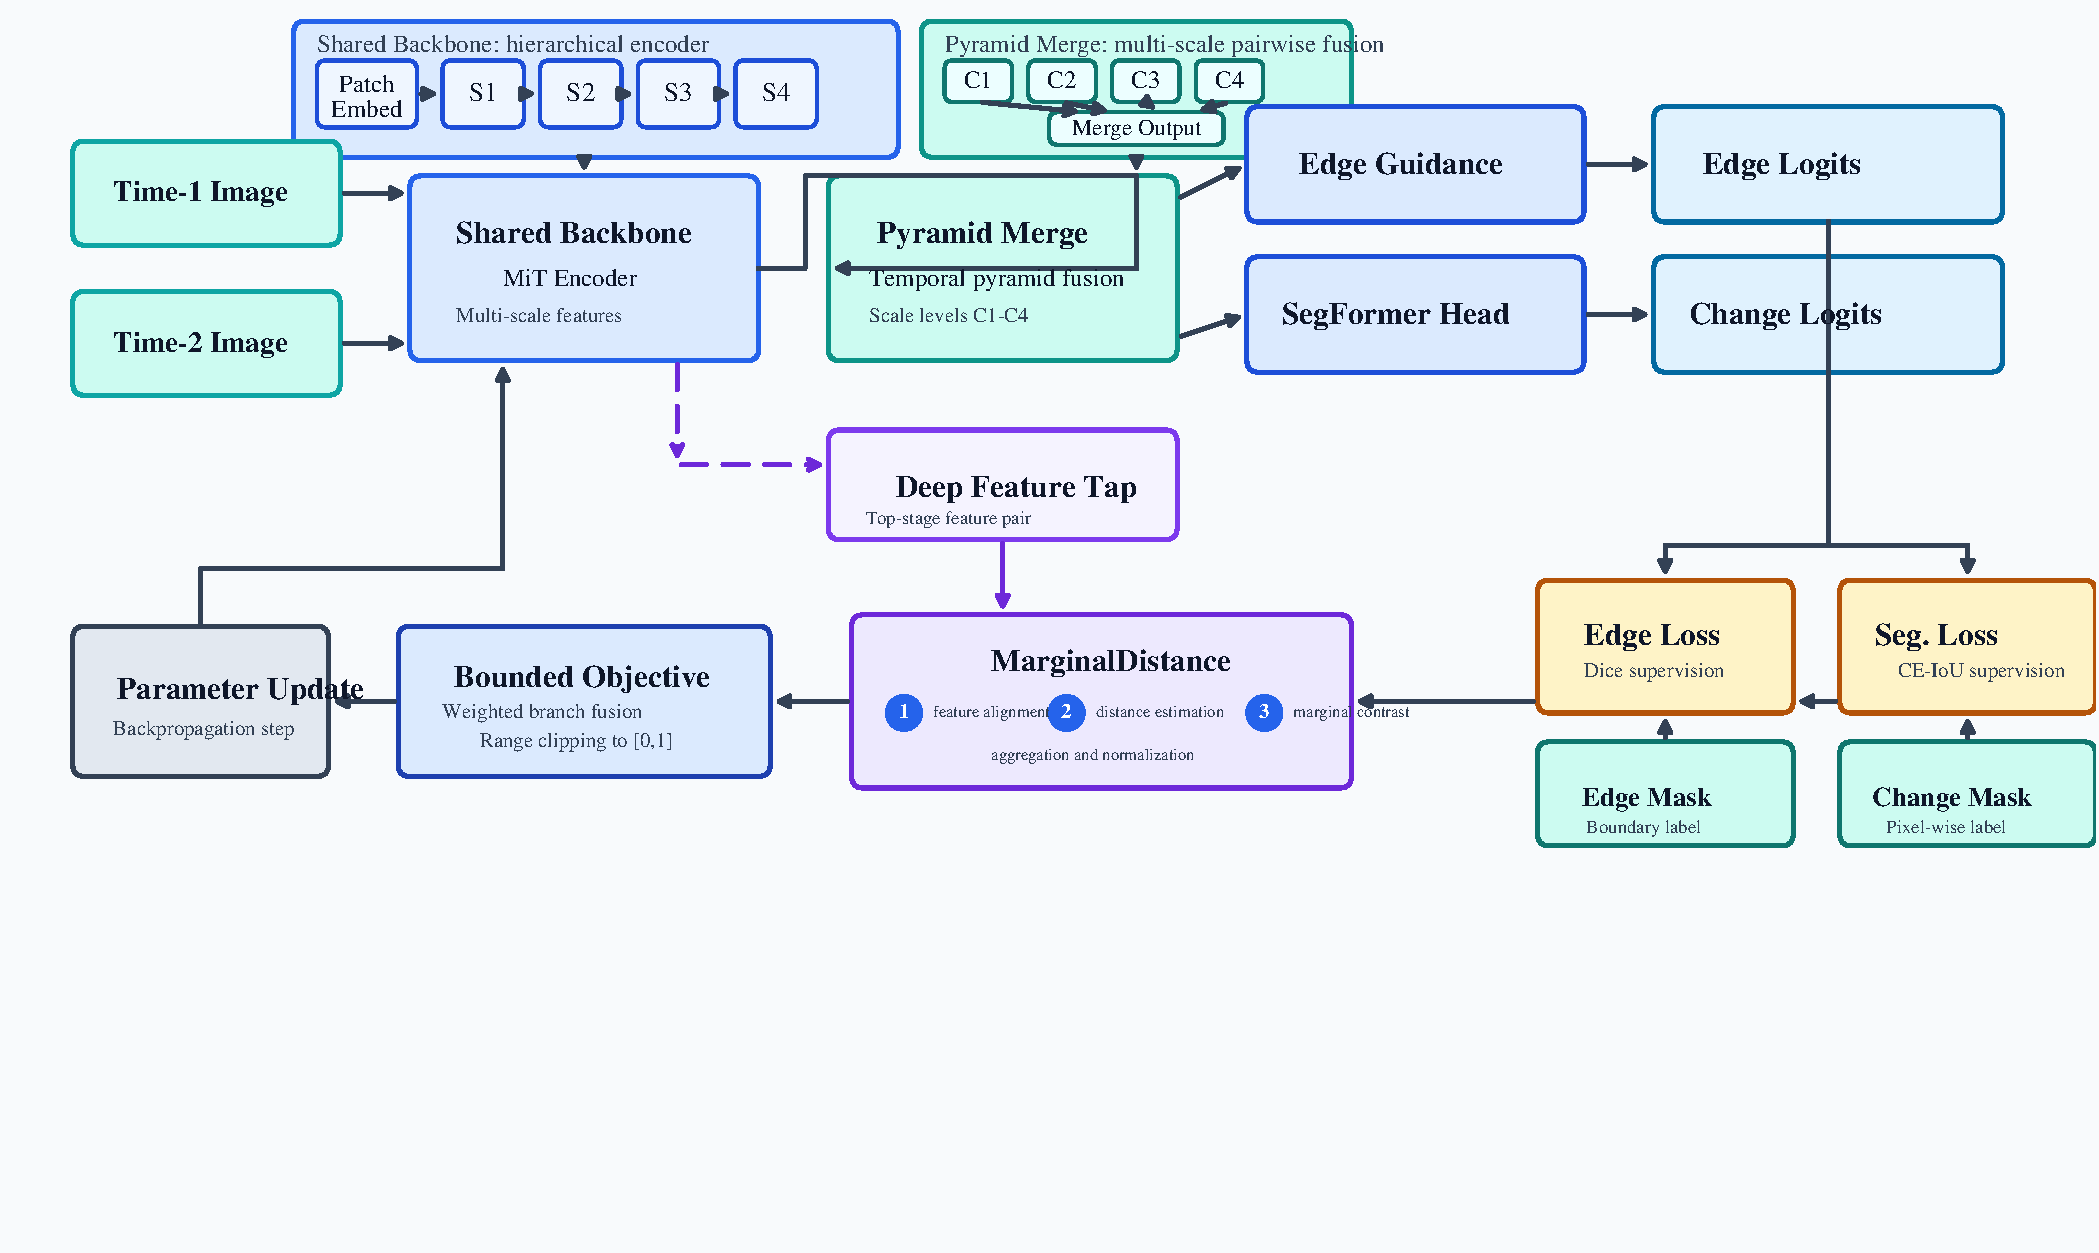
\includegraphics[width=0.98\textwidth]{Figures/overview_method_pipeline.pdf}
    \caption{Overall training pipeline of the proposed method. The model contains shared temporal encoding, pyramid-level fusion, dual prediction heads (change and edge), and a \textsc{MarginalDistance} branch for pseudo-change suppression. Multi-branch losses are bounded and fused to update network parameters.}
    \label{fig:method_overview}
\end{figure*}

Given bi-temporal images $\mathbf{I}^{t_1}$ and $\mathbf{I}^{t_2}$, the network $\mathcal{N}_{\theta}$ outputs change logits $\mathbf{P}$, edge logits $\mathbf{P}^{e}$, and deep features $\mathbf{F}^{t_1},\mathbf{F}^{t_2}$:
\begin{equation}
    \left(\mathbf{P},\mathbf{P}^{e},\mathbf{F}^{t_1},\mathbf{F}^{t_2}\right)
    =
    \mathcal{N}_{\theta}\left(\mathbf{I}^{t_1},\mathbf{I}^{t_2}\right).
    \label{eq:network_mapping}
\end{equation}

Following Fig.~\ref{fig:method_overview}, supervision is organized into three branches: segmentation (CE and IoU), edge prediction, and contrastive discrepancy modeling. Their normalized terms are finally fused into a bounded objective for stable multi-task optimization.

\subsection{Pseudo-Change Suppression via Label-Guided Contrastive Supervision}\label{sec:Methodology:PseudoChangeSuppression}
Let $(i,j)\in\Omega$ denote a pixel location, and let $\mathbf{F}^{t_1},\mathbf{F}^{t_2}\in\mathbb{R}^{C\times H\times W}$ be deep features from the two temporal inputs. We first apply channel-wise L2 normalization:
\begin{equation}
    \tilde{\mathbf{f}}^{t_1}_{ij}=
    \frac{\mathbf{F}^{t_1}_{ij}}{\left\|\mathbf{F}^{t_1}_{ij}\right\|_2},
    \qquad
    \tilde{\mathbf{f}}^{t_2}_{ij}=
    \frac{\mathbf{F}^{t_2}_{ij}}{\left\|\mathbf{F}^{t_2}_{ij}\right\|_2}.
    \label{eq:feature_normalization}
\end{equation}
Then the pixel-wise Euclidean distance is
\begin{equation}
    d_{ij}=\left\|\tilde{\mathbf{f}}^{t_1}_{ij}-\tilde{\mathbf{f}}^{t_2}_{ij}\right\|_2.
    \label{eq:feature_distance}
\end{equation}

With binary label $y_{ij}\in\{0,1\}$ ($0$: unchanged, $1$: changed), the pixel-wise contrastive penalty is
\begin{equation}
    \ell_{\text{con}}^{ij}
    =
    \frac{1-y_{ij}}{2}d_{ij}^{2}
    +
    \frac{y_{ij}}{2}\max(0,m-d_{ij})^{2},
    \label{eq:pixel_contrastive}
\end{equation}
where $m$ is the contrastive margin. Unchanged pixels are pulled closer, while changed pixels are pushed apart up to the margin.

The image-level contrastive loss is
\begin{equation}
    \bar{\mathcal{L}}_{\text{con}}
    =
    \frac{1}{HW}\sum_{i=1}^{H}\sum_{j=1}^{W}\ell_{\text{con}}^{ij},
    \label{eq:image_contrastive}
\end{equation}
and its bounded form is
\begin{equation}
    \mathcal{L}_{\text{con}}^{\text{norm}}
    =
    \operatorname{clip}
    \left(
        \frac{\bar{\mathcal{L}}_{\text{con}}}{\max\left(1,\frac{1}{2}m^2\right)},
        0,1
    \right).
    \label{eq:contrastive_normalization}
\end{equation}

\subsection{Objective Function}\label{sec:Methodology:ObjectiveFunction}
Following Table~\ref{tab:notations}, let $\mathbf{Y}$ be the change label map, $\mathbf{Y}^{e}$ be the edge label map, and $\theta$ be network parameters. The segmentation branch combines CE and IoU losses:
\begin{equation}
    \mathcal{L}_{\text{seg}}
    =
    \alpha\,\mathcal{L}_{\text{ce}}^{\text{norm}}
    +
    (1-\alpha)\,\mathcal{L}_{\text{iou}}^{\text{norm}},
    \label{eq:segmentation_fusion}
\end{equation}
with
\begin{equation}
    \mathcal{L}_{\text{ce}}^{\text{norm}}=1-\exp\left(-\mathcal{L}_{\text{ce}}\right),
    \label{eq:ce_normalization}
\end{equation}
\begin{equation}
    \mathcal{L}_{\text{iou}}^{\text{norm}}=\operatorname{clip}(\mathcal{L}_{\text{iou}},0,1),
    \qquad
    \mathcal{L}_{\text{edge}}^{\text{norm}}=\operatorname{clip}(\mathcal{L}_{\text{edge}},0,1).
    \label{eq:edge_iou_normalization}
\end{equation}

The fused multi-task objective is
\begin{equation}
    \mathcal{L}_{\text{total}}
    =
    (1-\beta-\gamma)\mathcal{L}_{\text{seg}}
    +
    \beta\mathcal{L}_{\text{con}}^{\text{norm}}
    +
    \gamma\mathcal{L}_{\text{edge}}^{\text{norm}},
    \label{eq:total_objective}
\end{equation}
subject to $0\le\beta\le1$, $0\le\gamma\le1$, and $\beta+\gamma\le1$. The final bounded loss is
\begin{equation}
    \mathcal{L}=\operatorname{clip}(\mathcal{L}_{\text{total}},0,1).
    \label{eq:final_objective}
\end{equation}

Accordingly, the optimization target is
\begin{equation}
    \theta^{*}
    =
    \arg\min_{\theta}
    \mathbb{E}_{\left(\mathbf{I}^{t_1},\mathbf{I}^{t_2},\mathbf{Y},\mathbf{Y}^{e}\right)}
    \left[\mathcal{L}\right].
    \label{eq:argmin_objective}
\end{equation}

\subsection{Algorithm: Annotation-Consistent Bounded Multi-Task Optimization}\label{sec:Methodology:Algorithm}
Algorithm~\ref{alg:proposed} gives the complete optimization routine. The algorithm explicitly includes forward mapping, contrastive subroutine, bounded loss fusion, and gradient update. Variable semantics are explained inline at first appearance so the flow remains self-explanatory.

\begin{algorithm}[t]
    \caption{Annotation-Consistent Bounded Multi-Task Optimization}
    \label{alg:proposed}
    \begin{algorithmic}[1]
        \Require bi-temporal images $\mathbf{I}^{t_1},\mathbf{I}^{t_2}$; change labels $\mathbf{Y}$; edge labels $\mathbf{Y}^{e}$; contrastive margin $m$; CE/IoU balance $\alpha$; branch weights $\beta,\gamma$; network parameters $\theta$
        \Ensure updated $\theta$ and final bounded loss $\mathcal{L}$
        \State Perform forward mapping to obtain $\mathbf{P}$, $\mathbf{P}^{e}$, $\mathbf{F}^{t_1}$, and $\mathbf{F}^{t_2}$ by Eq.~\eqref{eq:network_mapping}
        \State Compute $\mathcal{L}_{\text{con}}^{\text{norm}}$ using \textsc{MarginalDistance}$(\mathbf{F}^{t_1},\mathbf{F}^{t_2},\mathbf{Y},m)$
        \State Compute $\mathcal{L}_{\text{ce}}$, $\mathcal{L}_{\text{iou}}$, and $\mathcal{L}_{\text{edge}}$ as defined in Section~\ref{sec:Preliminary}
        \State Bound branch losses: $\mathcal{L}_{\text{ce}}^{\text{norm}}$ by Eq.~\eqref{eq:ce_normalization}; $\mathcal{L}_{\text{iou}}^{\text{norm}}$ and $\mathcal{L}_{\text{edge}}^{\text{norm}}$ by Eq.~\eqref{eq:edge_iou_normalization}
        \State Compute $\mathcal{L}_{\text{seg}}$ by Eq.~\eqref{eq:segmentation_fusion}
        \State Compute $\mathcal{L}_{\text{total}}$ by Eq.~\eqref{eq:total_objective}
        \State Compute final bounded loss $\mathcal{L}$ by Eq.~\eqref{eq:final_objective}
        \State Update $\theta$ via backpropagation with objective $\mathcal{L}$
        \Statex
        \Procedure{MarginalDistance}{$\mathbf{F}^{t_1},\mathbf{F}^{t_2},\mathbf{Y},m$}
            \State Define pixel-coordinate set $\Omega$
            \For{each $(i,j)\in\Omega$}
                \State Normalize $\mathbf{F}^{t_1}_{ij}$ and $\mathbf{F}^{t_2}_{ij}$ to unit vectors by Eq.~\eqref{eq:feature_normalization}
                \State Compute feature distance $d_{ij}$ by Eq.~\eqref{eq:feature_distance}
                \State Compute pixel penalty $\ell_{\text{con}}^{ij}$ by Eq.~\eqref{eq:pixel_contrastive} with label $y_{ij}\in\{0,1\}$
            \EndFor
            \State Average over pixels to obtain $\bar{\mathcal{L}}_{\text{con}}$ by Eq.~\eqref{eq:image_contrastive}
            \State Normalize and clip $\bar{\mathcal{L}}_{\text{con}}$ to $\mathcal{L}_{\text{con}}^{\text{norm}}$ by Eq.~\eqref{eq:contrastive_normalization}
            \State \Return $\mathcal{L}_{\text{con}}^{\text{norm}}$
        \EndProcedure
    \end{algorithmic}
\end{algorithm}
